% !TEX root = thesis.tex
\chapter{Web工学への深層学習技術の応用}
この章では、第4章で得られたDeep Learning用の構成を用いて、実際に機械学習のタスクを実行する。分類精度、実行時間、消費メモリ量を調べることにより、Deep LearningをWeb工学の問題に適用するe
際の参考とする。
\section{利用したデータセット}
実験の前提知識として、この節では、実験に使用したデータセットについて記す。機械学習の分野では、分類精度のベンチマークを取るために、様々なデータセットが提供/提案されてきている。同じデータセットに対して、様々な分類モデルやアルゴリズムを用いて分類実験を行うことにより、どの手法が優れているのか比較することが出来る。\par
ここでは、画像認識のデータセットを用いて、Deep Learningプログラムのベンチマークを行う。画像データを用いる理由は、1つには、画像認識がDeep Learningが最も高い分類性能を実現している分野だからである。加えて、画像データや画像から抽出された素性は、可視化が比較的容易なことが多い。可視化することで、学習過程を目で見て確かめることが出来るため、アルゴリズムの分析を行いやすい、という利点がある。
\subsection{MNIST}
MNIST database\footnote{http://yann.lecun.com/exdb/mnist/}とは、手書き数字を画像分析によって認識するベンチマークタスクである。このデータセットは、National Institute of Standards and Technology(NIST)が提供する手書き数字のデータにサイズの規格化処理を加え、数字の書き手毎に整理したものである。データはサイズ28x28ピクセルの白黒画像70000件より構成される\cite{lecun1998gradient-based}。それぞれの画像は、0〜9のいずれかの数字1文字に該当している。画像データを認識プログラムに入力して、どの数字に該当するか判別させることで、画像識別の精度を競うことになる。図\ref{c5_mnist_ex}に、MNISTの画像データの一部を示す(\cite{lecun1998gradient-based}より引用した)。\par
MNISTの70000件のデータは、60000件のモデル訓練用データと、10000件の精度測定用データに分かれている。まず60000件のデータを使って識別モデルに学習を行わせた後、未知の10000件のテストデータを実際に識別してみることで、精度を測定する。テストデータを識別している最中に、更なる学習を行うことは許されない。分類器は、過去に学習に使ったデータだけ良く識別できても意味がなく、むしろ未知のデータこそ精度良く分類出来なければならない。モデルが過去のデータに特化してしまうと、かえって未知のデータに対する識別精度が低下することもある。この低下現象は過学習(over fitting)と呼ばれ、機械学習における落とし穴の一つとなっている。MNISTに限らず、機械学習用のデータセットにて、訓練データとテストデータをあらかじめ分けておくことは一般的であり、学習アルゴリズムが過学習を防げているかどうか、判定するために有効な方法の1つとして知られている。\par
\begin{figure}[tbp]
 \begin{center}
  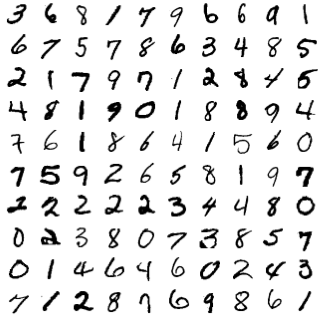
\includegraphics[width=50mm]{img/c5/mnist_ex}
 \end{center}
 \caption{MNISTデータの例}
 \label{c5_mnist_ex}
\end{figure}
MNISTは、様々な画像認識アルゴリズムの作者によって使用されている。MNISTの配布Webサイトには、MNISTを利用した論文のリストが、分類誤差によるランキング形式で掲載されている。表\ref{c5_mnist_rank}に、MNISTデータセットにおける各アルゴリズムの分類誤差を、ランキング形式のWebサイト\footnote{\label{c5_rank}\url{http://rodrigob.github.io/are_we_there_yet/build/classification_datasets_results.html}}より再構成して示す。

% Table generated by Excel2LaTeX from sheet 'c5mnist'
\begin{table}[htbp]
\begin{center}
  %\centering
  \caption{MNISTの分類誤差ランキング}
    \begin{tabular}{|l|l|r|}\hline
%    \toprule
    手法 & 発表学会/雑誌/年 & 分類誤差 \\ \hline
%    \midrule
    DropConnect \cite{wan2013regularization}& ICML 2013 & 0.21\% \\ \hline
    Multi-column Deep Neural Networks \cite{ciresan2012multi-column}& CVPR 2012 & 0.23\% \\ \hline
    Deep Big Simple Neural Nets \cite{ciresan2010deep}& Neural Computation 2010 & 0.35\% \\ \hline
    Energy-Based Model \cite{poultney2006efficient}& NIPS 2006 & 0.39\% \\ \hline
    Convolutional Neural Networks \cite{simard2003best}& Document Analysis and Recognition 2003 & 0.40\% \\ \hline
    \textbf{Maxout Networks} \cite{goodfellow2013maxout}& ICML 2013 & 0.45\% \\ \hline
    COSFIRE filters \cite{azzopardi2013trainable}& PAMI 2013 & 0.52\% \\ \hline
    Multi-Stage Architecture \cite{jarrett2009what}& ICCV 2009 & 0.53\% \\ \hline
    Deformation Models \cite{keysers2007deformation}& PAMI 2007 & 0.54\% \\ \hline
    A trainable feature extractor \cite{lauer2007a-trainable}& Journal Pattern Recognition 2007   & 0.54\% \\ \hline
    Invariant Support Vector Machines \cite{decoste2002training}& Machine Learning 2002 & 0.56\% \\ \hline
    Sparse Coding \cite{labusch2008simple}& TNN 2008 & 0.59\% \\ \hline
    Unsupervised learning of invariant feature hierarchies \cite{ranzato2007unsupervised}& CVPR 2007 & 0.62\% \\ \hline
    shape contexts \cite{belongie2002shape}& PAMI 2002 & 0.63\% \\ \hline
    Receptive Field Learning \cite{jia2012beyond}& CVPR 2012 & 0.64\% \\ \hline
    Sparse Activity, Sparse Connectivity \cite{thom2013sparse}& JMLR 2013 & 0.75\% \\ \hline
    Convolutional Deep Belief Networks \cite{lee2009convolutional}& ICML 2009 & 0.82\% \\ \hline
    Deep Encoder Network \cite{min2009large-margin}& 2009 & 0.94\% \\ \hline
    Deep Boltzmann Machines \cite{salakhutdinov2009deep}& AISTATS 2009 & 0.95\% \\ \hline
    Deep Belief Networks \cite{dahl2008cs81:}& 2008 & 1.12\% \\ \hline
    Convolutional Neural Networks  \cite{simard2003best}& 2003 & 1.19\% \\ \hline
    neural networks \cite{hinton2006reducing}& 2006 & 1.20\% \\ \hline
    Deep learning via semi-supervised embedding \cite{weston2012deep}& 2008 & 1.50\% \\ \hline
%    \bottomrule
    \end{tabular}%
  \label{c5_mnist_rank}%
  \end{center}
\end{table}%

\subsection{CIFAR10}
CIFAR10\footnote{http://www.cs.toronto.edu/~kriz/cifar.html}は、写真を画像分析によって識別するタスクである\cite{krizhevsky2009learning}。入力データは60000件のカラー画像で、どの画像も、飛行機、自動車、鳥、猫、鹿、犬、蛙、馬、船、トラックの10種類のクラスのどれかに属しており、各クラス均等に6000枚ずつの画像が割り振られている。画像データは、GoogleやFlickrなどによるWeb検索で集められた画像を、人手でラベリングして作られている。また、サイズを32x32ピクセルに縮小されている。\par
MNISTと同じように、60000件のデータは、50000の訓練データと10000件のテストデータに分割されている。まず、分類器にこれらの訓練データを読み取らせて、学習を行わせる。その後、テストデータのうちいくつを正しいクラスに分類することができるのか、分類精度を競うことになる。\par
CIFAR10についても、データの例を\ref{c5_cifar_ex}に、分類誤差のランキングWebサイト\footnote{\url{http://rodrigob.github.io/are_we_there_yet/build/classification_datasets_results.html}}より、再構成した表を\ref{c5_cifar_rank}に示す。
\begin{figure}[tbp]
 \begin{center}
  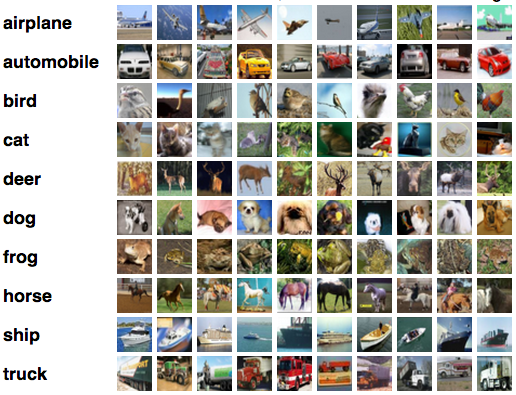
\includegraphics[width=100mm]{img/c5/cifar_ex}
 \end{center}
 \caption{CIFAR10データの例}
 \label{c5_cifar_ex}
\end{figure}
\begin{table}[tbp]
 \begin{center}
  \begin{tabular}{|l|l|r|}\hline
  手法 & 発表学会/雑誌 & 分類誤差 \\ \hline
DropConnect \cite{wan2013regularization}& ICML 2013 & 9.32 \% \\ \hline
Maxout Networks \cite{goodfellow2013maxout}& ICML 2013 & 9.35 \% \\ \hline
Bayesian Optimization \cite{snoek2012practical}& NIPS 2012 & 9.50 \% \\ \hline
Deep Convolutional Neural Networks \cite{krizhevsky2012imagenet}& NIPS 2012 & 11.00 \% \\ \hline
Multi-Column Deep Neural Networks \cite{ciresan2012multi-column}& CVPR 2012 & 11.21 \% \\ \hline
Deep Convolutional Neural Networks \cite{zeiler2013stochastic}& arXiv 2013 & 15.13 \% \\ \hline
Dropout \cite{hinton2012improving}& arXiv 2012 & 15.60 \% \\ \hline
Sum-Product Networks \cite{gens2012discriminative}& NIPS 2012 & 16.04 \% \\ \hline
Single-Layer Networks \cite{coates2011an-analysis}& AISTATS 2011 & 20.4 \% \\ \hline
  \end{tabular}
 \end{center}
 \caption{CIFAR10分類誤差のランキング}
 \label{c5_cifar_rank}
\end{table}

\section{使用したライブラリ}
この章の実験には、pylearn2というDeep Learningのライブラリを用いた。
\section{使用したハードウェア}
この章の実験では、GPUを搭載したサーバマシンを用いた。表\ref{c5_hardware_spec}に、今回の実験で使用したマシンの主な使用パーツ及び性能を列挙した。また、Maxout Networkの実装ソースコードには、実験マシンのパーツ性能を書いたファイルが付属している\footnote{pylearn2/scripts/papers/maxout/notes}。このファイルの記述内容も、比較のために列挙した。今回の実験に使ったマシンの方が、ハードウェア性能的には優れていることがわかる。
\begin{table}[tbp]
 \begin{center}
  \begin{tabular}{|c|c|c|c|c|c|}\hline
   & GPU & CUDA core & CPU & クロック数 & メモリ容量\\ \hline
今回 & GTX760 & 1152 & Intel CPU Core i7 4770S & 3.1 GHz & 32GB\\ \hline
論文 & GTX580 & 512 & Intel Xeon CPU E5620 &  2.40GHz & (記載無し)\\ \hline
  \end{tabular}
 \end{center}
 \caption{ハードウェア性能の比較}
 \label{c5_hardware_spec}
\end{table}

\section{ベンチマーク実験の詳細}
前節で挙げた画像分類のベンチマークセットに対し、Deep Learningの様々なアルゴリズムによって分類を行わせ、その性能を測定した。

\subsection{Maxout Networkによる、MNISTの分類タスク(2次元データとして扱う)}
Maxout Networkを分類器として用い、MNISTの分類タスクを行わせた。モデル構造としては、Convolutional Layerを2層重ねた上に、全てのニューロンが単純に接続されたMaxout Layerを1層付け加え、最後の層にてロジスティック回帰を行って分類結果を出した。
実験を行った結果、分類誤差は0.51\%となった。これは、元の論文が主張している分類誤差より、僅かに悪い結果となった。
\begin{table}[tdp]
\caption{Maxout NetworkによるMNIST(2次元)分類の結果}
\begin{center}
\begin{tabular}{|c|c|c|c|c|}\hline
手法 & データセット & 元論文の誤差 & 実験誤差 & 増加分\\ \hline
Maxout Network & MNIST(2次元) & 0.45\% & 0.51\% & +0.06\% \\ \hline
\end{tabular}
\end{center}
\label{c5_maxout_mnist1_result}
\end{table}%

\subsection{Maxout Networkによる、MNISTの分類タスク(1次元データとして扱う)}
前項と同じタスクを、「MNISTのデータは、2次元の画像データではなく、1次元のベクトルデータである」という条件の基で行わせた。つまり、2次元データに対するConvolutional Layer技術を敢えて使わない状態で、どれだけの精度をMaxout Networkが実現できるのか、実験した。この条件でもMaxout Networkが良い性能を出すことが出来れば、1次元のデータ、例えば言語データや音声データにおいても、Maxout Networkが応用できる可能性が高くなる。\\
また、何らかの原因でランダム性が発生していないか確かめるため、この実験は同じ条件で10回行った。乱数のシードは、元論文の実験が行われたときと同じ値で固定した。\\
実験の結果、誤差は10回とも共通で、1.16\%となった。Maxoutの元の論文やはり少し低い精度になってしまった(表\ref{c5_maxout_mnist1_result})。なお、平均実行時間は55分、最大メモリ使用量は793MBだった(表\ref{c5_maxout_mnist1_stat})。\\
\begin{table}[tdp]
\caption{Maxout NetworkによるMNIST(1次元)分類の結果}
\begin{center}
\begin{tabular}{|c|c|c|c|c|}\hline
手法 & データセット & 元論文の誤差 & 実験誤差 & 増加分\\ \hline
Maxout Network & MNIST(1次元) & 0.94\% & 1.16\% & +0.12\% \\ \hline
\end{tabular}
\end{center}
\label{c5_maxout_mnist1_result}
\end{table}%

\begin{table}[tdp]
\caption{Maxout NetworkによるMNIST(1次元)分類の実験詳細}
\begin{center}
\begin{tabular}{|c|c|c|}\hline
 & 平均実行時間(秒) & 平均最大使用メモリ(MB) \\ \hline
pretraining & 2532.8 & 779.3 \\ \hline
finetuning & 756.7 & 792.5 \\ \hline
全体 & 3289.5 & 792.5 \\ \hline
\end{tabular}
\end{center}
\label{c5_maxout_mnist1_stat}
\end{table}%


\subsection{Maxout Networkによる、CIFAR10の分類タスク}
データセットを変更し、MNISTではなく、CIFAR10をMaxout Networkを用いて分類させようと試みた。データは2次元画像として扱った。つまり、Convolutional Layerの使用は可能とした。レイヤー構造は、Convolutional Layer 3層 - Maxout Layer1層 - 識別用Softmax Layer1層とした。\par
しかし、この実験を実際に行ったところ、3日間実行を続けたところで、残りエポック数と計算速度の比較より、全体の実行が完了するまでに10日以上かかることが判明した。これはWeb工学における応用に使う学習アルゴリズムとして、試行錯誤しながら使うものとしては現実的でない実行時間である。また、実験スケジュールの都合もあり、実験の中断を余儀なくされてしまった。実行が完了した部分までの分類誤差を、図??に示した。[図追加]